\subsection{Native: goal-aware, viability-gated self-evolution}
\label{sec:native}

% Role: motivation. Message: a supplied measurement need not exhaust the objective.
Native studies self-evolution when the objective is not necessarily identical to an external score. A natural-language goal can be fully operationalized by a benchmark, or only partly measured by it. The default protocol asks the harness to judge that relationship and to add or revise its own tests when useful. It does not mandate extra tests or treat a self-reported score as an independent measurement. The legacy interface also permits a goal without an evaluator, or open-ended exploration without a supplied goal; those are explicit settings rather than evidence of autonomous capability growth.

% Role: method. Message: the running harness proposes changes to its own declared state.
The reference episode uses \emph{observe, propose, act, reflect}. The active harness inspects its state and permitted evidence, chooses a scoped change, edits its pending candidate, and records outcomes and unresolved risks. The four phase names alone are not the contribution. The relevant experimental choices are which goal and evidence are supplied, what state the harness can change, which implementation executes each phase, and how a candidate becomes active. For supported staged-source adapters, all phases run the frozen last-valid source, including reflection; pending edits take effect only after validation and activation. Self-authored tests remain part of the harness state, distinct from the external grader.

% Role: formalization. Message: the common profile has an explicit non-score admission rule.
The common-contract profile separates the active harness $A_t$ from the working candidate $W_t$. For an episode that completes successfully and publishes a candidate, let it produce $\widetilde W_{t+1}=F_\theta(A_t,W_t,G,V_t)$, where $G$ is the supplied goal, $V_t$ is permitted evidence, and the model weights $\theta$ remain fixed. With a model-free viability check $v$, its transition is
\begin{equation}
 W_{t+1}=\widetilde W_{t+1},\qquad
 A_{t+1}=\begin{cases}
 \widetilde W_{t+1}, & v(\widetilde W_{t+1})=1,\\
 A_t, & v(\widetilde W_{t+1})=0.
 \end{cases}
\label{eq:native-transition}
\end{equation}
There is no condition requiring an external score to increase. A viable candidate becomes active even if its measured task score decreases; an invalid candidate remains the exact working state for a later repair episode while execution retains $A_t$. An actor/stage failure or an uncertain external operation stops this transition and follows the shared failure/recovery protocol; it is not silently treated as a viability rejection. This defines a continuation policy, not a monotonic-improvement guarantee. The final candidate is the last valid one, not an outer-loop score maximum.

\begin{figure}[t]
\centering
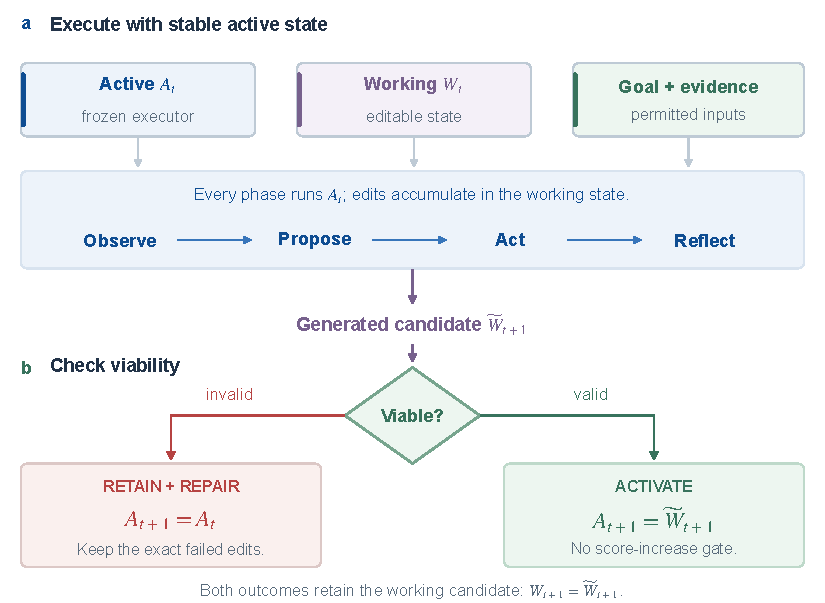
\includegraphics[width=\linewidth]{figures/native-transition.pdf}
\caption{\textbf{Native common-profile transition.} The current active harness executes the episode while changes accumulate in a separate working candidate. A source-bound viability result controls activation. Completed but nonviable edits remain available for repair, and formal scores enter later reasoning only through the declared evidence policy; they do not implement an outer acceptance filter. This figure describes supported staged-source execution, not every legacy adapter's lifecycle.}
\label{fig:native}
\end{figure}

% Role: scope. Message: the two Native profiles must not be conflated.
The common profile requires observed evaluation pools, evaluates the initial and each viable candidate, and runs optional hidden tests after evolution. It binds evolution and subject roles to the same harness integration and uses exactly one managed episode stage. Its supported phase controls do not make it an arbitrary stage graph. Legacy Native retains its separate goal/no-goal options, evaluator schedules, dispositions, measurements, and selection settings. Accordingly, the no-outer-score rule in Equation~\ref{eq:native-transition} describes the common profile; it must not be generalized to every legacy configuration.

% Role: evidence and limitation. Message: current evidence supports the mechanism, not its advantage.
The source-bound Native fixture demonstrates invalid-edit retention, later repair, changed candidate execution, private final grading, and replay. Bounded Pi/DSH pilots additionally exercise one common episode; the broader engineering record tests supported source activation paths. These support the implemented state transition. They do not establish that goal-aware self-evolution beats score-guided search, that self-authored tests are useful, or that useful improvements compound. Such claims require matched comparisons varying objective framing, evidence access, activation/selection policy, and self-evidence while holding tasks, models, initial artifacts, and budgets fixed.
